\section{Method}
\label{sec:benchmark}
\benchmark{} evaluates autonomous multimodal post-training through a controlled research environment and three complementary evaluation dimensions (Figure~\ref{fig:protocol}). We describe the task setting and evaluation protocol before introducing our proposed research framework, \harness{}.

\begin{figure}[t]
\centering
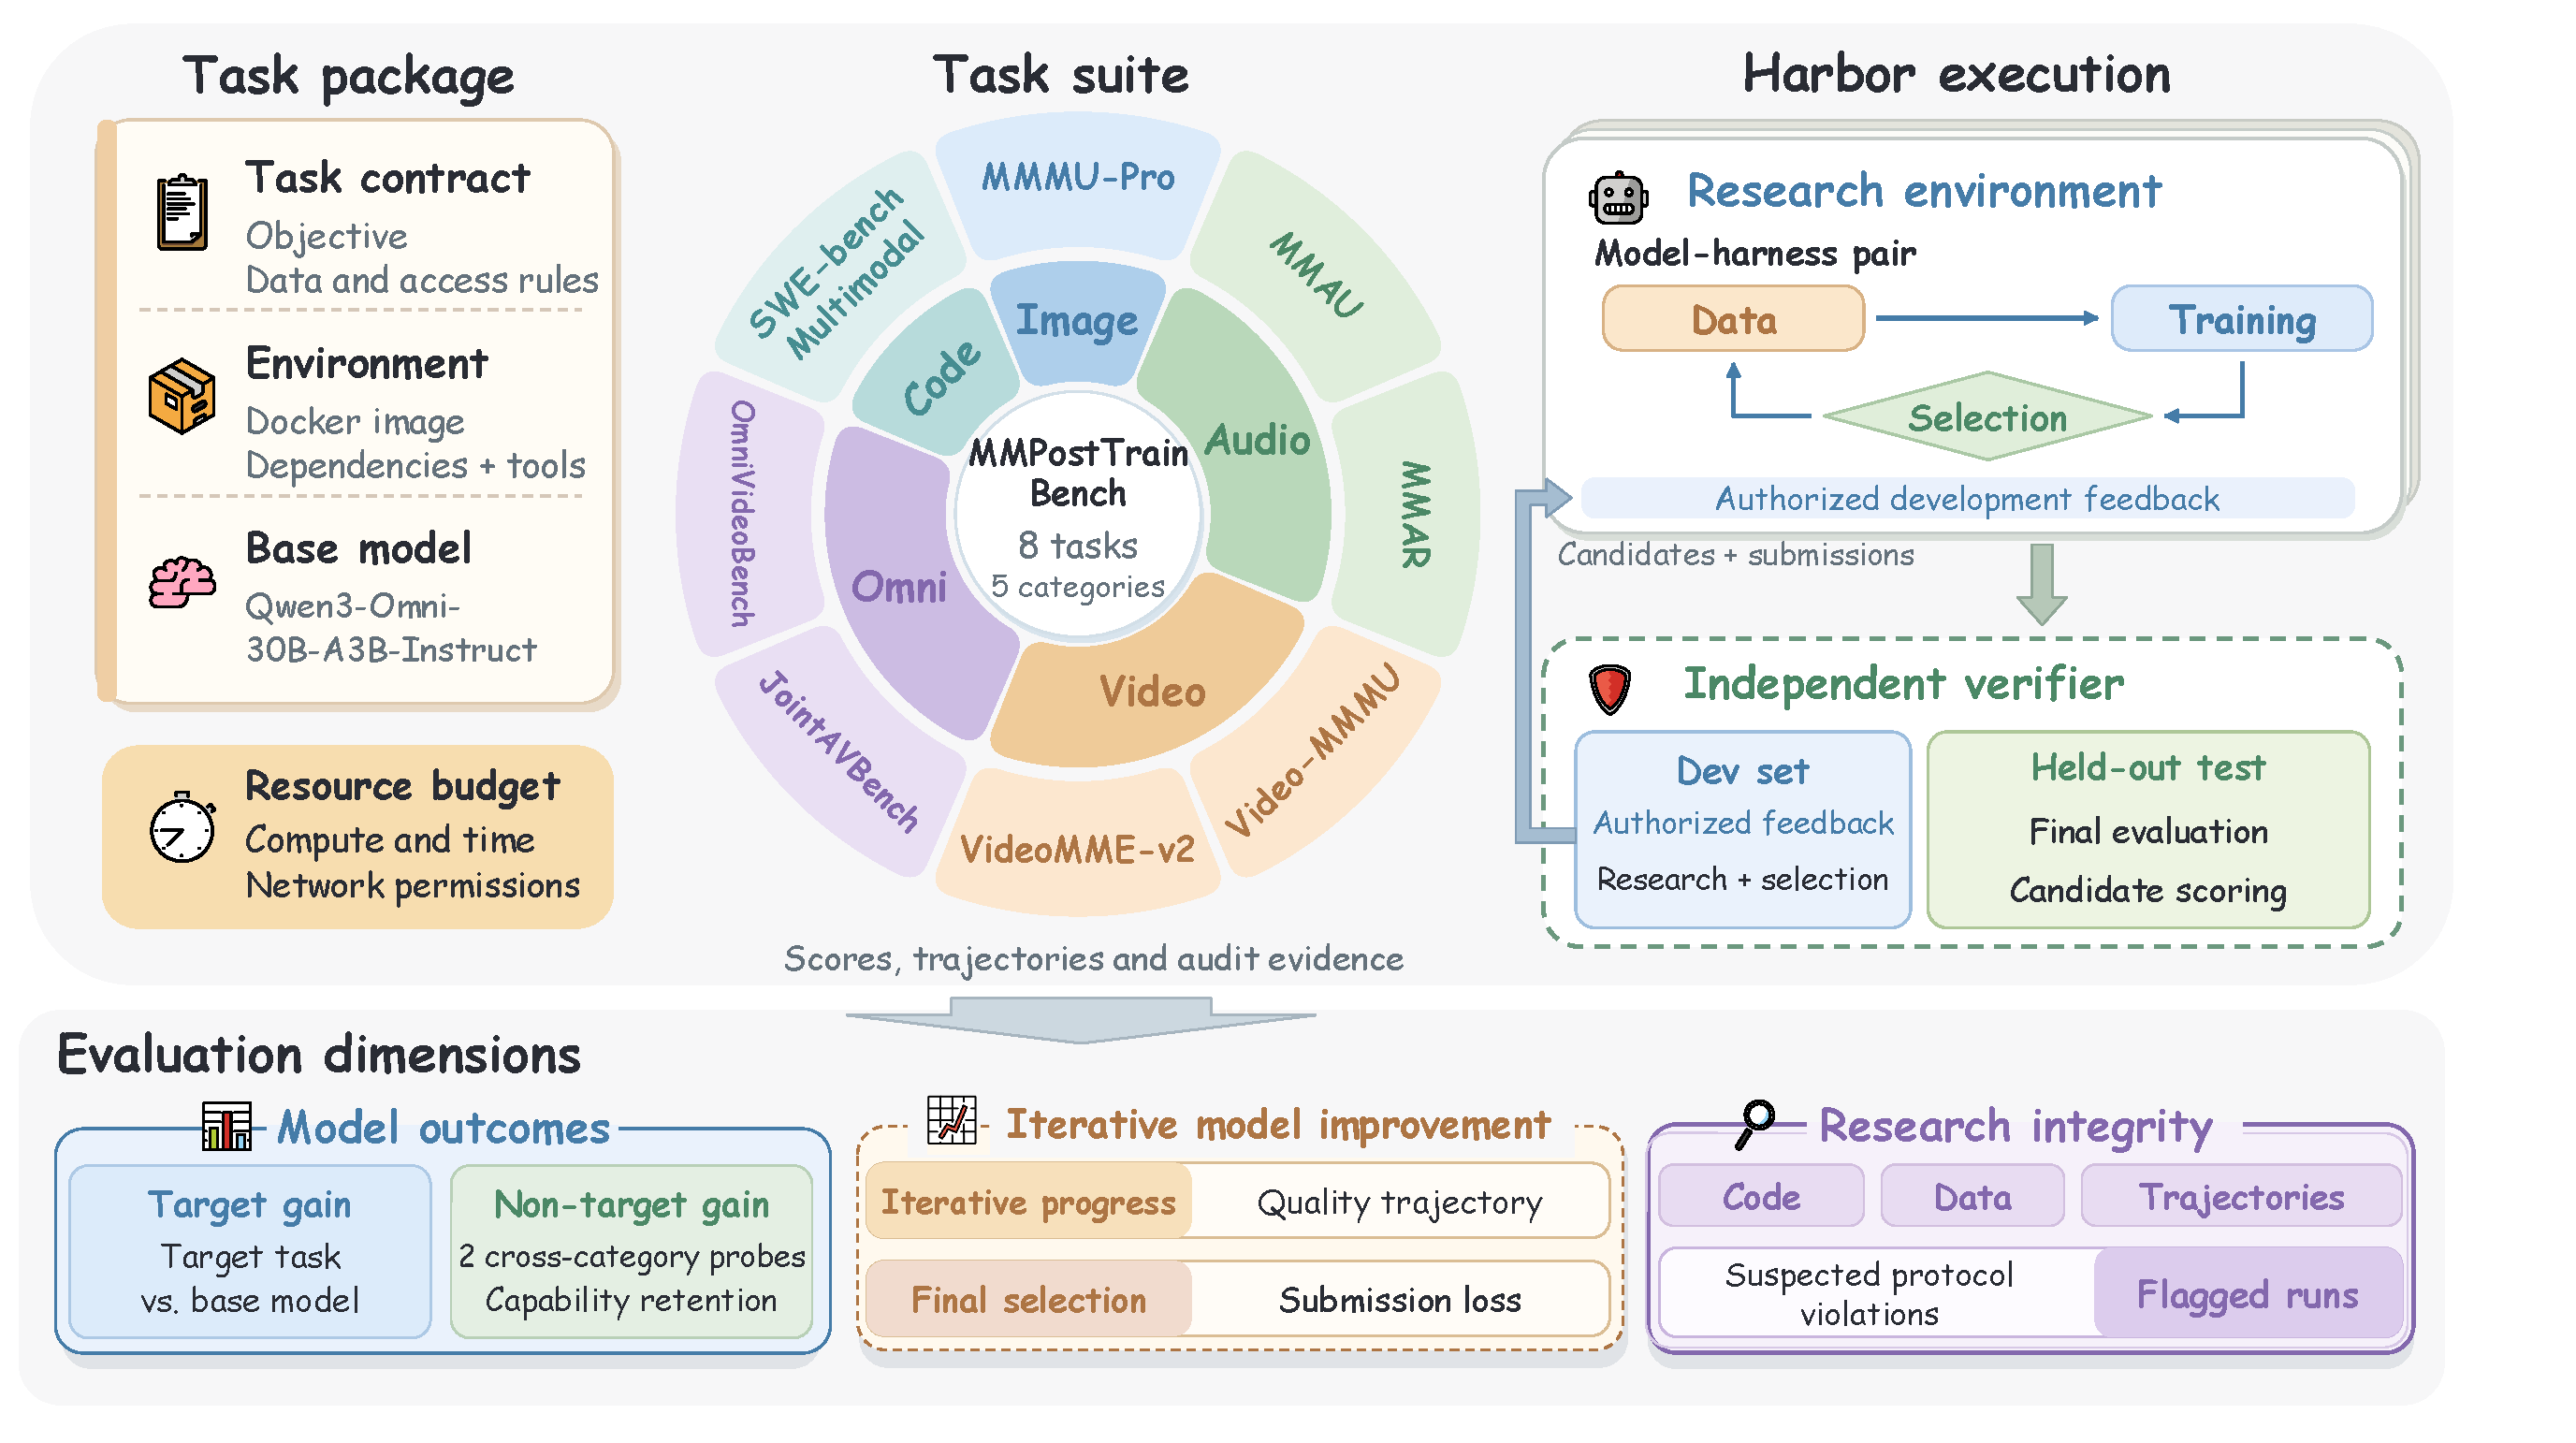
\includegraphics[width=1.0\linewidth]{mile/figures/benchmark_overview_v20.pdf}
\caption{\textbf{MMPostTrainBench benchmark overview.} Agents conduct post-training from a common base model on eight multimodal tasks within fixed budgets. To limit evaluation leakage, execution and verification run in separate containers, research feedback is restricted to authorized development data, and final tests remain sealed. Submitted models, candidate trajectories, and audits support evaluation of model outcomes, iterative model improvement, and research integrity.}
\label{fig:protocol}
\end{figure}

\subsection{Task Definition and Research Process}
\label{sec:task-definition}
\paragraph{Research task.}
A task assigns the agent a capability to improve, a starting model, and a bounded research environment. Following the artifact-oriented setup of autonomous post-training and research benchmarks~\citep{posttrainbench,rsibenchdata,arbor}, we represent task $b$ as
\begin{equation}
\mathcal{T}_b=(q_b,\theta_0,\mathcal{D}^{\mathrm{adm}}_b,F_b^{\mathrm{dev}},E_b^{\mathrm{test}},\mathcal{B}_b).
\label{eq:research-task}
\end{equation}
Here $q_b$ specifies the target capability and success criterion; $\theta_0$ is the common base model; $\mathcal{D}^{\mathrm{adm}}_b$ specifies permitted training-data sources and uses; $F_b^{\mathrm{dev}}$ returns authorized development feedback; $E_b^{\mathrm{test}}$ independently evaluates frozen models; and $\mathcal{B}_b$ specifies compute allocation and the research time limit. Research configuration $a$ consists of a frontier model and its execution runtime.

\paragraph{Autonomous research.}
Within loop $r$, the agent chooses interventions from its accumulated history rather than following a prescribed training recipe. Suppressing $a,b,r$ for clarity, candidate production and feedback can be written as
\begin{align}
u_t&=\pi_a(q_b,\mathcal{H}_{<t}), &
\theta_t&=\operatorname{Execute}(u_t;\theta_0,\mathcal{C}_{<t}),\nonumber\\
f_t&=F_b^{\mathrm{dev}}(\theta_t), &
\mathcal{H}_{\le t}&=\mathcal{H}_{<t}\cup\{(u_t,\theta_t,f_t,\ell_t)\}.
\label{eq:research-process}
\end{align}
An intervention $u_t$ specifies data construction, a training recipe, or a model-side operation using permitted prior candidates $\mathcal{C}_{<t}$; $\ell_t$ records execution diagnostics and provenance. The initial history contains permitted task materials, and later observations include only information available during research. The agent decides how many experiments to attempt and which completed model $S_{a,b,r}=\theta^{\mathrm{sub}}_{a,b,r}$ to submit before the budget expires.

\begin{table}[!htbp]
\centering\renewcommand{\arraystretch}{1.15}\small
\setlength{\tabcolsep}{4pt}
\caption{Eight post-training tasks, their domains, and target model abilities.}
\label{tab:tasks}
\begin{tabular}{@{}lll@{}}
\toprule
Task & Domain & Model Ability \\
\midrule
MMMU-Pro~\citep{mmmupro} & Image & Image-grounded multidisciplinary reasoning \\
\addlinespace[3pt]
MMAU~\citep{mmau} & Audio & Audio understanding and reasoning \\
MMAR~\citep{mmar} & Audio & Audio reasoning \\
\addlinespace[3pt]
Video-MMMU~\citep{videommmu} & Video & Video-grounded multidisciplinary reasoning \\
VideoMME-v2~\citep{videommev2} & Video & Video understanding \\
\addlinespace[3pt]
JointAVBench~\citep{jointavbench} & Omni & Joint audio-video understanding \\
OmniVideoBench~\citep{omnivideobench} & Omni & Joint audio-video understanding and reasoning \\
\addlinespace[3pt]
SWE-bench Multimodal~\citep{swebench_multimodal} & Code & Image-grounded software repair \\
\bottomrule
\end{tabular}
\end{table}

%
%


\subsection{Research Environment and Protocol}
\label{sec:environment}
\paragraph{Task environment.}
Each Harbor-compatible task package specifies the task objective, designated base model, data-use rules, tool interfaces, and resource limits. The research environment provides a writable workspace and the dependencies required for model training and evaluation. Within the task's permissions, agents can inspect multimodal media, construct training examples, modify training code and configurations, execute experiments, and retain candidate models. Harbor's separate-verifier interface and the Docker driver separate research execution from independent verification.

\paragraph{Development feedback.}
Agents query $F_b^{\mathrm{dev}}$ to obtain candidate scores, permitted evaluation examples, and execution diagnostics. These observations support error diagnosis and subsequent decisions about data construction, training configurations, and candidate selection. The task's data-use rules determine which materials may serve as training supervision; access to evaluation examples for diagnosis does not itself authorize their use for training. Development feedback excludes final held-out test instances, reference answers, and scores, which remain withheld during research.

\paragraph{Submission and verification.}
At the end of research, the selected model's weights, configuration, and loading dependencies are frozen and transferred to the independent verifier. The final evaluator $E_b^{\mathrm{test}}$ assesses the base and submitted models using the same fixed held-out test instances, preprocessing, inference interface, and scoring procedure. This matched evaluation provides the basis for measuring changes in model performance. Data provenance, tool traces, and candidate records connect the submitted model to its research process and support the integrity checks defined in Section~\ref{sec:evaluation-dimensions}.

\subsection{Evaluation Dimensions}
\label{sec:evaluation-dimensions}
We evaluate three complementary dimensions: model outcomes, iterative model improvement, and research integrity. Let $S=\theta^{\mathrm{sub}}_{a,b}$ denote the submitted model and $H_b(\theta)\in[0,1]$ its raw task score: answer accuracy for understanding tasks and resolved-instance rate for SWE-bench Multimodal.

\noindent\textbf{Model outcomes.}
We compare submissions with the base on the target task and two prespecified non-target probes from other categories. Target change is $\Delta_{a,b}=100[\widehat{s}_{a,b}-H_b(\theta_0)]$ percentage points, where $\widehat{s}_{a,b}$ is the mean of three loop scores, with flagged loops reset to the base before averaging. Non-target changes assess transfer and capability retention. Aggregate comparisons weight all eight tasks equally. For SWE-bench Multimodal, Table~\ref{tab:main} reports submitted-model means relative to a base resolved-instance rate of 2.29\%.

\noindent\textbf{Iterative model improvement.}
We assess iterative model improvement from two perspectives. \textbf{(1) Iterative progress:} whether further experiments improve candidate quality or lead to stagnation, degradation, or fluctuations, as reflected by candidate trajectories evaluated retrospectively on the same held-out test set. \textbf{(2) Final selection:} whether the final submission retains the best performance among the evaluated candidates produced before submission. Let $\mathcal{C}^{\mathrm{rec}}_{a,b}$ denote this candidate set. Submission loss is defined as
\begin{equation}
R^{\mathrm{rec}}_{a,b}=100\!\left[\max_{\theta\in\mathcal{C}^{\mathrm{rec}}_{a,b}\cup\{S\}}H_b(\theta)-H_b(S)\right].
\label{eq:submission-loss}
\end{equation}
A positive value indicates that the final submission underperforms the best evaluated candidate, with the gap measured in percentage points.

\noindent\textbf{Research integrity.}
Benchmark scores may be inflated by contamination or misuse of evaluation information. Audit categories cover training-data contamination, unauthorized workspace or data access, prohibited split use, and misuse of evaluation information. Retained code, data provenance, and research trajectories provide evidence for these checks. Results are summarized by the number of runs flagged for suspected violations.

\subsection{MMResearch: Multimodal Research Framework}
\label{sec:harness}
\harness{} adds a research controller to existing code-agent runtimes, retaining their native tools and action loops while coordinating experiments, memory, and model delivery. Figure~\ref{fig:harness} shows how hierarchical memory (a) and multimodal evidence (c) support the seven-step research loop (b), which concludes with model delivery (d). The evidence-anchor and graph design in (c) specifies how localized media observations connect to research hypotheses and experimental outcomes.

\begin{figure}[t]
\centering
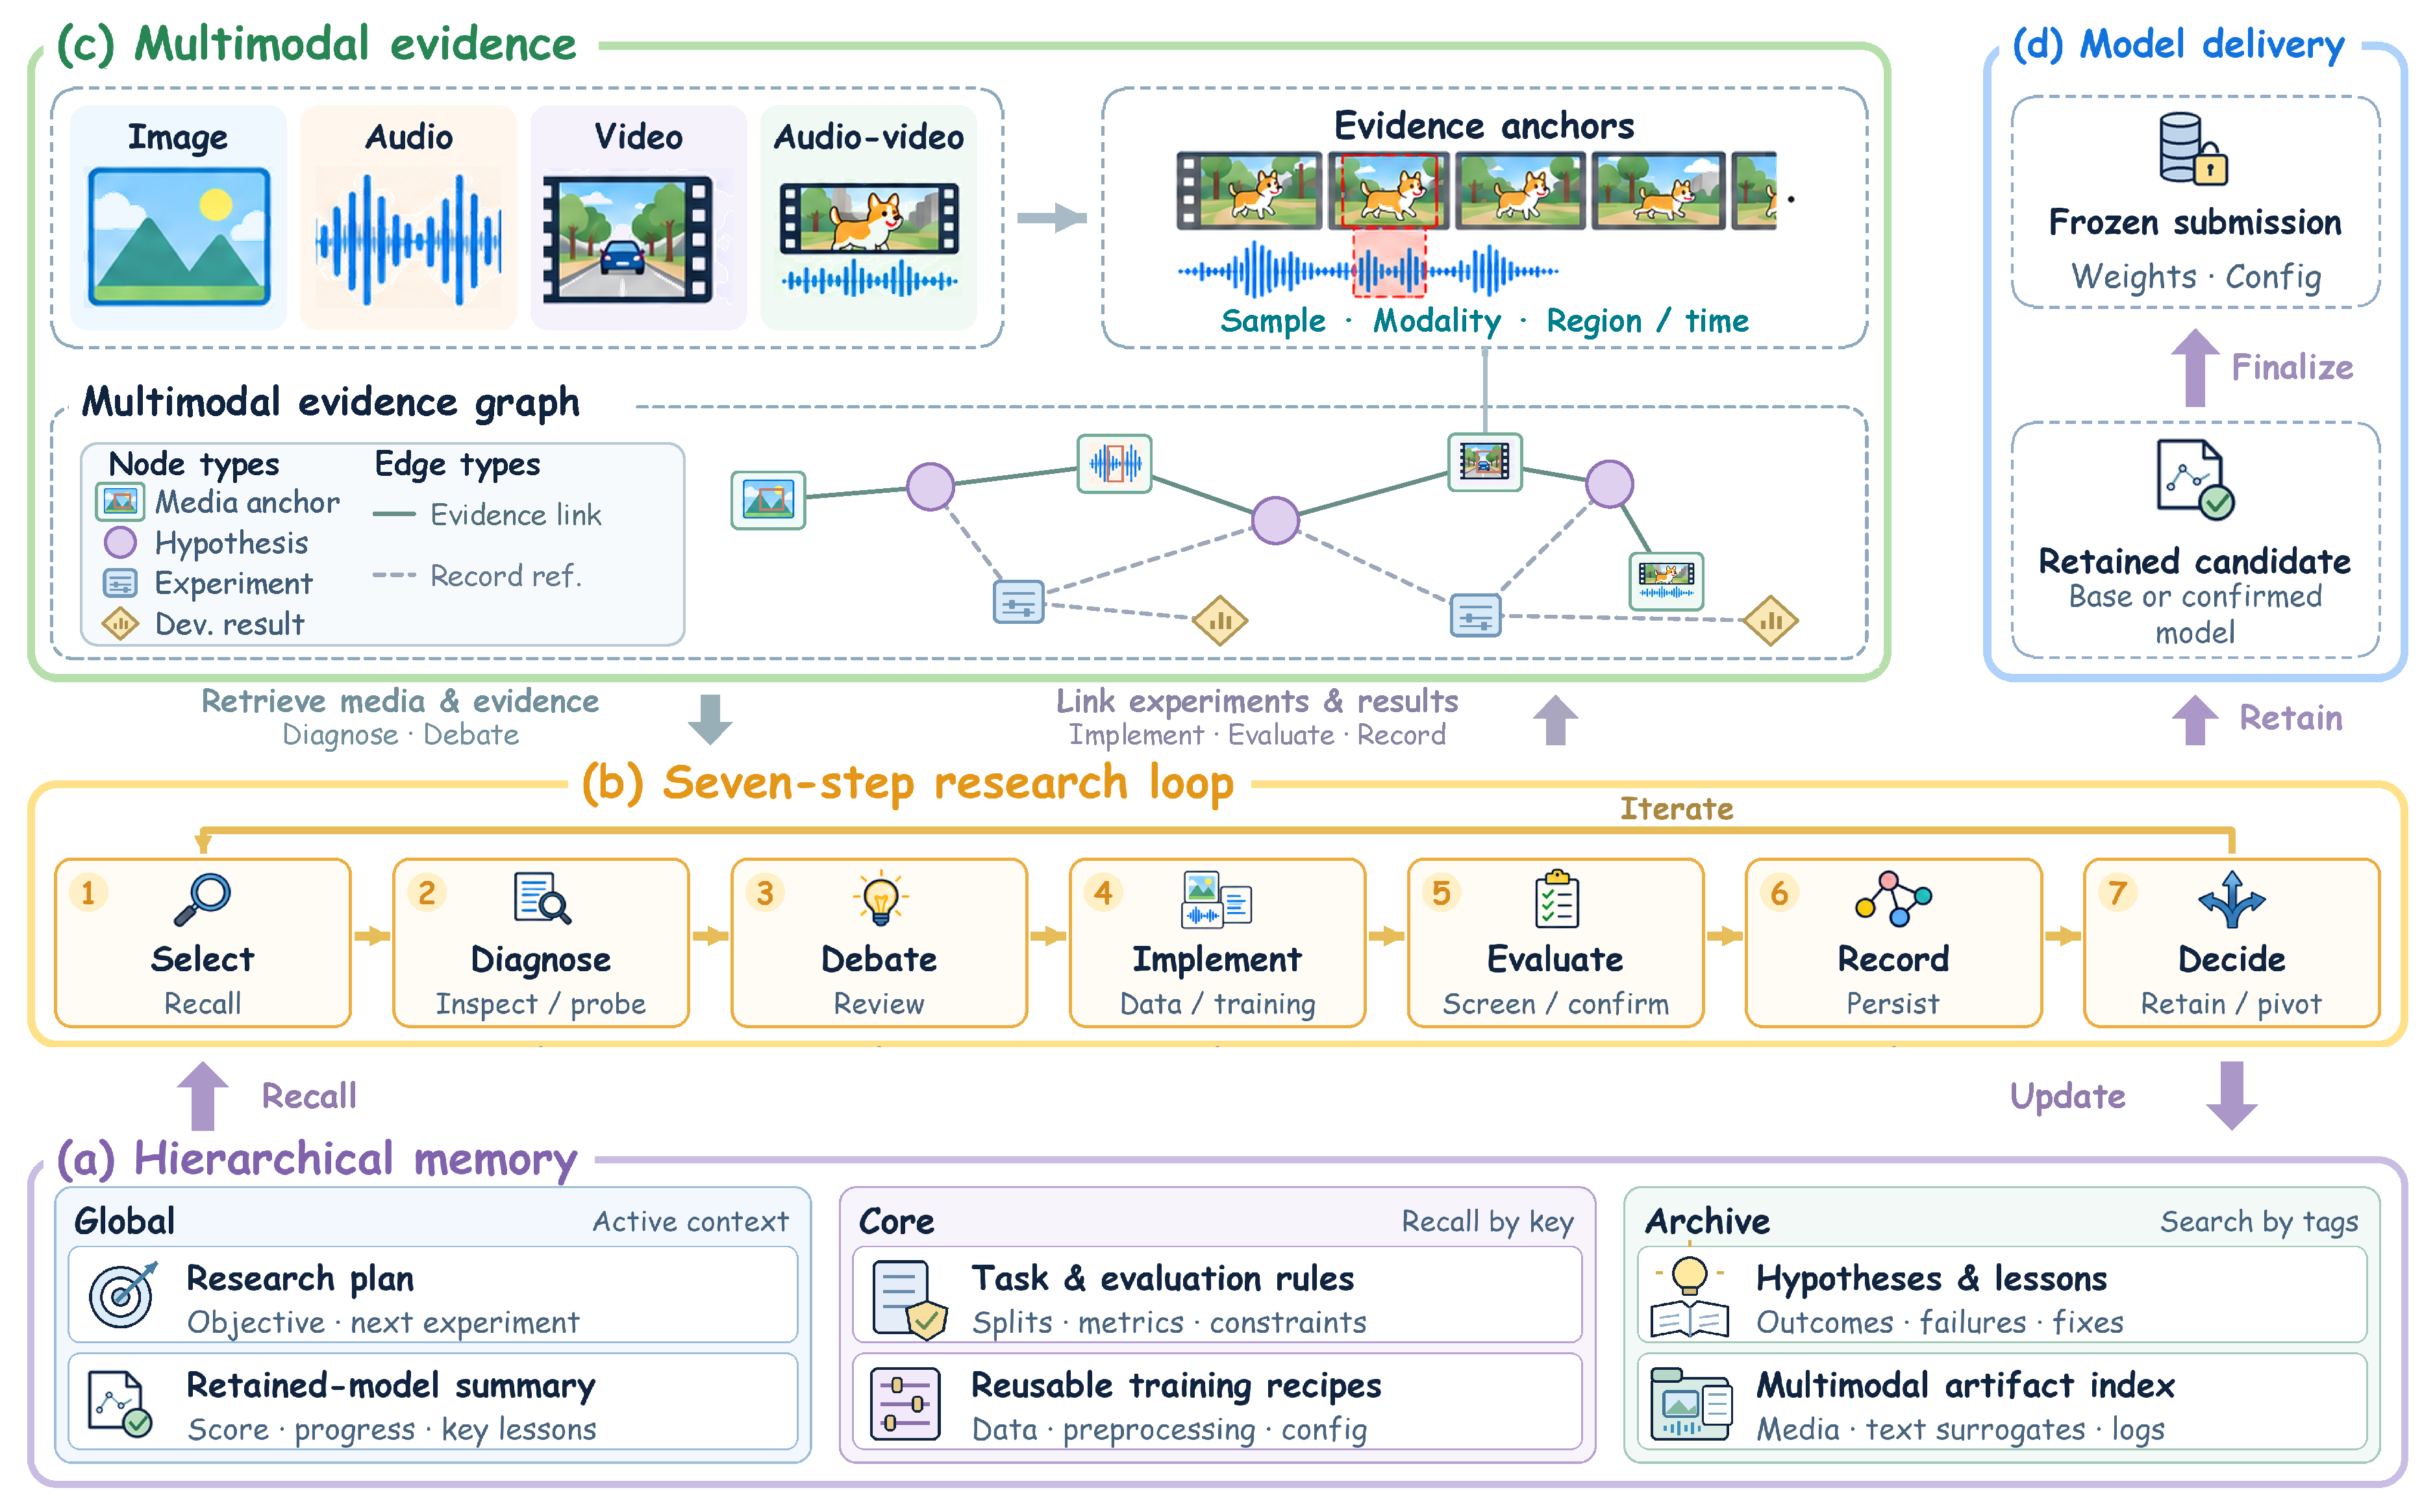
\includegraphics[width=1.0\linewidth]{mile/figures/reference_harness.pdf}
\caption{\textbf{MMResearch framework.} MMResearch coordinates a seven-step research loop (b), using hierarchical memory (a) to guide experimentation and multimodal evidence (c) to connect observations with experimental decisions, then freezes the retained candidate for delivery (d).}
\label{fig:harness}
\end{figure}

\noindent\textbf{Seven-Step Research Loop.}
Each round turns a research direction into an evaluated candidate and a decision (Figure~\ref{fig:harness}b). \textsc{Select} chooses a data- or model-side direction from prior hypotheses and failure records. \textsc{Diagnose} inspects authorized multimodal inputs to investigate the suspected failure. \textsc{Debate} reviews the diagnosis, intervention, feasibility, and risks. \textsc{Implement} executes the intervention and saves a candidate. \textsc{Evaluate} screens and confirms candidates on development data. \textsc{Record} stores configurations, results, and rationales in hierarchical memory. \textsc{Decide} uses confirmation results to promote the candidate, refine the approach, or pivot to another direction; a proxy improvement alone does not justify promotion. A separate checkpoint tracks the retained model, initially the base. Before the budget expires, the controller checks required records and freezes the retained model's weights and configuration for delivery.

\noindent\textbf{Multimodal Evidence.}
The agent inspects authorized image, audio, video, and audio-video inputs through native perception or configured tools. In the \emph{multimodal evidence graph} design (Figure~\ref{fig:harness}c), each \emph{evidence anchor} identifies a source sample, its modality, and a relevant region or time span. When finer localization is unavailable, the anchor refers to the whole image or clip. Direct observations are stored separately from the hypotheses inferred from them. Links connect observations, hypotheses, training interventions, and development-evaluation outcomes, making diagnoses traceable to the underlying media. \textsc{Diagnose} and \textsc{Debate} use the linked observations to review explanations; \textsc{Record} preserves the evidence and outcome links for subsequent rounds. Later rounds can follow these links back to the source media and prior interventions to reassess an earlier diagnosis in light of development results. Held-out test results remain outside this research feedback loop.

\noindent\textbf{Hierarchical Memory.}
\harness{} preserves research context across rounds in three memory tiers (Figure~\ref{fig:harness}a). \emph{Global} maintains the active research plan and a summary of the retained model. \emph{Core} stores task and evaluation rules and reusable training recipes. \emph{Archive} indexes hypotheses, outcomes, failures, and media artifacts. \textsc{Select} retrieves relevant records at the start of a round, and \textsc{Record} updates them with its results and lessons, allowing later experiments to build on earlier findings.


